\documentclass[UTF8,a4paper,11pt,twocolumn]{ctexart}
\usepackage{amsmath,amsfonts,amssymb}
\usepackage{booktabs}
\usepackage{graphicx}
\usepackage{fancyhdr} %设置页眉页脚

\pagestyle{fancy}
\lhead{亚硫酸钠法处理含铬废液}
\rhead{\thepage}
\cfoot{}
\renewcommand{\headrulewidth}{0.4pt}

\begin{document}
\title{{\heiti 亚硫酸钠法处理含铬废液}}
\author{{\kaishu 刘宇杰}\\{\kaishu (南京大学匡亚明学院\quad 江苏\space 南京\quad 210046)}}
\date{}

\twocolumn[
\maketitle %maketitle必须添加在这里,否则摘要会跳转到下一页
\renewcommand{\abstractname}{}
\begin{abstract}
\noindent{}\textbf{摘要: }本文主要介绍实验室中含铬废液处理的方法——亚硫酸钠法,并对实验中易发生的胶体沉淀穿滤现象进行分析。在此基础上设计条件实验,探究不同絮凝剂对于沉淀过滤以及实验结果的影响,总结得出在沉淀形成之前加入钙盐可有效减少穿滤现象,获得较好的实验结果。\\
\noindent{}\textbf{关键词: }铬;亚硫酸钠;废液处理
\end{abstract}

\bigskip
\bigskip

\begin{center}
\large{\textbf{Using Sodium Sulfite to Treat Waste Liquid Containing Chromium}}\\
\normalsize{Liu Yujie}\\
(Nanjing University\quad Kuang Yaming Honors School\quad Jiangsu Nanjing\quad 210046)\\
\end{center}

\textbf{Abstract: }This paper mainly introduces the method of treating waste liquid containing chromium in the laboratory - sodium sulfite method and analyzes the phenomenon of colloid precipitation filtration which is easy to occur in the experiment. On this basis, a condition experiment was designed to explore the effect of different flocculants on the precipitation filtration. It was concluded that adding calcium salt before precipitation formation could effectively reduce the filtration phenomenon and obtain better experimental results.\\
\textbf{Key words: }Chromium; Sodium sulfite; Liquid waste processing

\bigskip
\bigskip
]

\begin{center}
{\heiti {\Large 引言}}
\end{center}

随着绿色化学理念的深入人心,实验室废液废物的处理也日趋重要。实验室中洗涤量器会使用到铬酸洗液,制备产品会用到重铬酸钾等等。这些过程中产生的含铬废液若不能正确处理,会对环境和人体造成巨大危害。铬被人体吸收后能导致头痛、贫血、消化障碍以及肾脏损害。更有甚者,六价铬的毒性比三价铬大100倍。若水中六价铬的含量大于0.1$mg/L$,就会对人体产生毒害作用。目前,处理含铬废水的主要方法有化学还原法,离子变换法,电解法,活性炭处理法,蒸发浓缩法以及电渗析法等。

\section{实验目的}
\begin{enumerate}
\item 学会使用氧化还原法、沉淀法去除某离子
\item 熟练掌握分光光度计的使用、工作曲线的绘制等
\item 学会自主设计实验,并能对实验结果进行分析并设计相应的条件实验
\item 了解绿色化学的基本理念,做到实验污染最小化,保护环境
\end{enumerate}

\section{实验原理}
\subsection{含铬污水处理常用方法}
\subsubsection{$SO_2$还原法}
二氧化硫处理后六价铬含量可达到0.l $mg/L$ 。但二氧化硫是有害气体,对操作人员有影响,处理池需用通风没备,另外对设备腐蚀性较大,不能直接回收铬酸。烟道气中的二氧化硫处理含铬(VI)废水,充分利用资源,以废治废,节约了处理成本,但也同样存在以上的问题。其反应原理为: 
{\small $$3SO_2 + Cr_2O^{2-}_7 + 2H^+ = Cr^{3+} + 3SO^{2-}_4 + H_2O $$}
{\small $$Cr^{3+} + 3OH^- = Cr(OH)_3$$}

\subsubsection{铁氧体法}
铁氧体法实际上是硫酸亚铁法的发展,向含铬废水中投加废铁粉或硫酸亚铁时,$Cr^{6+}$ 可被还原成 $Cr^{3+}$。再加热、加碱、通过空气搅拌,便成为铁氧体的组成部分,$Cr^{3+}$转化成类似尖晶石结构的铁氧体晶体而沉淀。铁氧体是指具有铁离子、氧离子及其他金属离子所组成的氧化物。其具体反应为: 
{\small $$Cr_2O_7^{2-} + 6Fe^{2+} + 14H^+ = 2Cr^{3+} + 6Fe^{3+} + 7H_2O$$}
{\footnotesize $$Fe^{2+} + Fe^{3+} + Cr^{3+} + O_2 = Fe^{3+}[Fe^{2+} Cr^{3+}_x Fe^{2+}_{1-x}]O_4$$}

铁氧体法不仅具有还原法的一般优点,还有其特点,即铬污泥可制作磁体和半导体,这样不但使铬可以回收利用,又减少了二次污染的发生,出水水质好,能达到排放标准。但是,铁氧体法也有试剂投量大,能耗较高,处理成本较高的缺点。 

\subsubsection{铁屑铁粉处理法}
铁屑铁粉由于原料易得,价格便宜,处理含铬(VI)等重金属废水效果较好,但该法要消耗较多的酸,同时污泥量较大,铁屑处理含铬废水有多种作用:

\begin{itemize}
\item 还原作用,由于铁屑中含有杂质,它们与铁的电位不同,铁作为阳极溶解,给出电子成为二价铁离子,电子转移到阴极被$Cr_2O_7^{2-}$ 和 $H^+$接受成为 $Cr^{3+}$和 $H_2$, 阴极生成的二价铁离子又将 $Cr_2O_7^{2-}$ 还原;
\item 置换作用,废水中电位比铁正的金属离子与金属铁屑粉末发生置换作用;
\item 凝聚作用,反应生成的氢氧化铁本身就是一种凝聚剂,有利于最后氢氧化铬等的沉降;
\item 中和作用,由于反应中要消耗大量的酸,随着反应进行 $pH$ 值不断升高,使 $Fe$ 呈氢氧化铁析出。 
\end{itemize}

\subsubsection{钡盐法}
利用溶度积原理,向含铬废水中投加溶度积比铬酸钡大的钡盐或钡的易溶化合物,使铬酸根与钡离子形成溶度积很小的铬酸钡沉淀而将铬酸根除去。废水中残余 $Ba^{2+}$再通过石膏过滤,形成硫酸钡沉淀,再利用微孔过滤器分离沉淀。反应式是: 
{\small $$BaCO_3 + H_2CrO_4= BaCrO_4+ CO_2 + H_2O$$}
{\small $$Ba^{2+} +CaSO_4 = BaSO_4 + Ca^{2+}$$}

钡盐法优点是工艺简单,效果好,处理后的水可用于电镀车间水洗工序,还可回收铬酸,复生 $BaCO_3$;其缺点是过滤用的微孔塑料管加工比较复杂,容易阻塞,清洗不便,处理工艺流程较为复杂。 

\subsubsection{电解还原法}
电解还原法是铁阳极在直流电作用下,不断溶解产生亚铁离子,在酸性条件下,将 $Cr^{6+}$还原为 $Cr^{3+}$。 用电解法处理含铬废水,优点是效果稳定可靠,操作管理简单,设备占地面积小,废水中的重金属离子也能通过电解有所降低。缺点是耗电量较大,消耗钢板,运行费用较高,沉渣综合利用等问题有待进一步解决。 

\subsubsection{离子交换法}
离子交换法是借助于离子交换剂上的离子和水中的离子进行交换反应除去水中有害离子。目前在水处理中广泛使用的是离子交换树脂。对含铬废水先调 $pH$ 值,沉淀一部分 $Cr^{3+}$后再行处理。将废水通过 $H$型阳离子交换树脂层,使废水中的阳离子交换成$H^+$而变成相应的酸,然后再通过 $OH$ 型阴离子交换成 $OH^-$,与留下的$H^+$结合生成水。吸附饱和后的离子交换树脂,用 $NaOH$ 进行再生。 离子交换法的优点是处理效果好,废水可回用,并可回收铬酸。尤其适用于处理污染物浓度低、水量小、出水要求高的废水。缺点是工艺较为复杂,且使用的树脂不同,工艺也不同;一次投资较大,占地面积大,运行费用高,材料成本高,因此对于水量很大的工业废水,该法在经济上不适用。

\subsection{二苯碳酰二肼比色法原理}
在酸性溶液中,六价铬离子与二苯碳酰二肼反应,生成紫红色络合物,其最大吸收波长为$540nm$,吸光度与浓度的关系符合比尔定律。反应式如下:
{\tiny $$(C_6H_5NHNH)_2CO + Cr^{6+} = C_6H_5(NH)_2CON_2C_6H_5 + Cr^{3+}$$}

\subsection{亚硫酸钠处理含铬废液原理}
在酸性条件下,向含铬废水中投入还原剂亚硫酸钠,使水中的六价铬还原成三价铬,调节废水至$pH = 8-9$ ,使三价铬生成难溶的氢氧化铬沉淀除去。

具体离子方程式如下:
{\small $$Cr_2O_7^{2-} + 3SO_3^{2-} + 8H^+ = 2Cr^{3+} + 3SO_4^{2-} +4H_2O$$}
{\small $$2Cr^{3+} + 3OH^- = Cr(OH)_3 \downarrow$$}

在反应中 {\small $n(Cr_2O_7^{2-}):n(SO_3^{2-})=1:3$},即{\small $n(Cr(VI)):n(Na_2SO_3)=2:3$}。所以我们一开始先用分光光度计测出废液中六价铬的含量,便可以计算出所需$Na_2SO_3$的质量:{\small $m(Na_2SO_3)=1.5×n(Cr(VI))×M(Na_2SO_3)$}。其中{\small $M(Na_2SO_3)=126.04g/mol$}

经实验表明,加入1.5倍理论值$^{[1]}$的$Na_2SO_3$可获得较好的还原效果。

\section{初次实验}
\subsection{实验仪器与试剂}
722型分光光度计、25mL比色管2套、移液枪、铬储备液(100$mg/L$)、废液、浓硫酸 [上海凌峰化学试剂有限公司 AR]、浓磷酸 [国药集团化学试剂有限公司 AR]、30\% 过氧化氢溶液 [南京化学试剂一厂 AR]、氢氧化钠固体 [国药集团化学试剂有限公司 AR]、亚硫酸钠固体、二苯碳酰二肼显色剂
\subsection{实验过程}
\subsubsection{Cr(VI)工作曲线的绘制}
取7支25mL比色管,用移液枪依次加入0、1、2、4、8、16、20mL Cr(VI)标准溶液(1$mg/L$),加入20滴1:1硫酸和20滴1:1磷酸,1.5mL显色剂,用纯水稀释至标线,摇匀。静置5min后,由浓度从低到高倒入比色皿中,选择波长$540nm$,测量吸光度,绘制工作曲线。
\subsubsection{原废液中Cr(VI)含量测定}
取1mL原废液,稀释至100mL,再从中取1mL,稀释至100mL,此即稀释10000倍的原液。从中取出10mL,置于25mL比色管中,加入20滴1:1硫酸和20滴1:1磷酸,1.5mL显色剂,用纯水稀释至标线,摇匀。测吸光度,由工作曲线求出浓度。
\subsubsection{还原}
取稀释5倍的原液50mL置于250mL烧杯中,调节$pH=1-2$,根据测得六价铬含量加入计算量的$Na_2SO_3$ ,反应迅速进行,溶液变成蓝绿色,此时还原反应基本结束。
\subsubsection{沉淀与处理}
在上述溶液加入$NaOH$固体(后期可加入浓溶液),调节$pH$=8-9,此时产生大量沉淀,加热陈化15min。冷却,加入适量活性炭,搅拌,吸滤,保留滤液。
\subsubsection{处理后六价铬和总铬含量测定}
取处理后溶液20mL,置于25mL比色管中,加入20滴1:1硫酸和20滴1:1磷酸,1.5mL显色剂,用纯水稀释至标线,摇匀。测吸光度,由工作曲线计算六价铬浓度。

调节处理后溶液$pH=12-13$,加入1-2滴30\% 过氧化氢溶液,将三价铬转化为六价铬。加热除去过量过氧化氢,取10mL,置于25mL比色管中,加入20滴1:1硫酸和20滴1:1磷酸使溶液呈酸性,加入1.5mL显色剂,用纯水稀释至标线,摇匀。测吸光度,由工作曲线计算总铬浓度。
\section{初次实验结果与分析}
\subsection{工作曲线的绘制(λ=540nm)}
见表1、图1。

\begin{table*}[h]
\centering
\begin{tabular}{cccccccc}
\toprule
标准液用量 $mL$&0&1&2&4&8&16&20\\
\midrule
浓度 $mg/L$&0&0.04&0.08&0.16&0.32&0.64&0.8\\
吸光度&0.003&0.033&0.069&0.118&0.253&0.504&0.622\\
\bottomrule
\end{tabular}
\caption{工作曲线}
\end{table*}

\begin{figure*}[h]
\centering
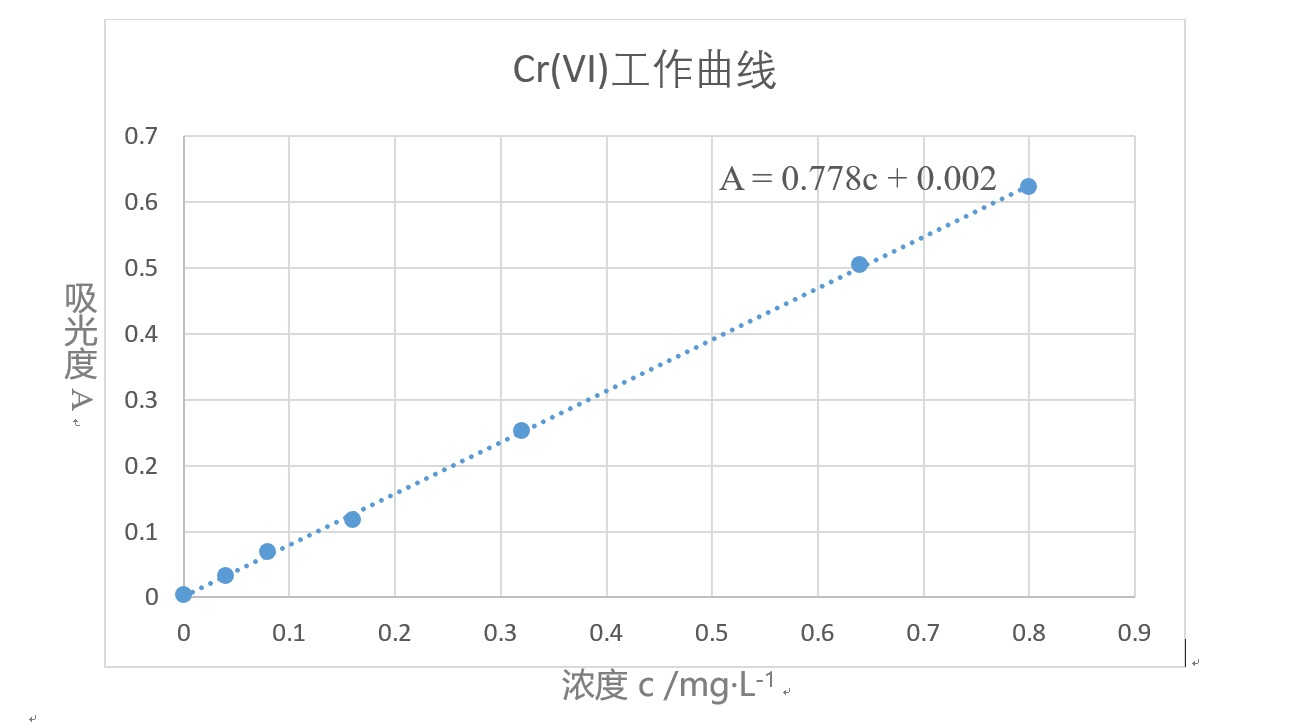
\includegraphics[scale=0.6]{gz.jpg}
\caption{工作曲线}
\end{figure*}

\subsection{原废液中Cr(VI)含量测定}
\begin{center}
25000倍稀释原液\space A=0.102\\原液\space c=3213 $mg/L$\\处理液\space c=642.6 $mg/L$
\end{center}
\subsection{计算m($Na_2SO_3$)、还原、沉淀}
$$m(Na_2SO_3)_{calculated}=0.16g$$
$$m(Na_2SO_3)_{used}=0.21g$$
$$m(NaOH)_{used}=8.3g$$
\subsection{处理后Cr(VI)、总Cr含量}
\begin{center}
(1.25倍稀释处理液\space A=0.013)\\计算得:六价铬\space c=0.018 $mg/L$\\
(2.50倍稀释处理液\space A=0.800)\\计算得:总铬量\space c=2.564 $mg/L$
\end{center}
\subsection{实验结果分析}
实验用亚硫酸钠作为还原剂,从实验结果可以看出,还原剂的效果很好,处理后溶液中六价铬含量很低。但是与之形成鲜明对比的是总铬含量超标多倍,远大于国标排放浓度0.5$mg/L$。其中的原因主要是形成的$Cr(OH)_3$沉淀呈胶体状,过滤时易穿滤,即便是加了活性炭对其进行了吸附也不能彻底解决穿滤问题。相比之下,使用铁氧体法的同学,其沉淀由于形成了铁氧体,在陈化之后过滤,穿滤现象比使用亚硫酸钠的同学要好一些。穿滤过去的细小的$Cr(OH)_3$胶体肉眼不可见,然而在测总铬时由于调节$pH>12$,导致$Cr(OH)_3$溶解,进而三价铬离子被双氧水氧化为六价铬离子,导致总镉含量超标。

在这种情况下,我们设计条件实验,探究不同的絮凝剂对于沉淀过滤的影响,并对结果进行分析与评估。

\section{条件实验方案设计}
在保持初次基本实验条件不变的情况下,对活性炭进行更换,分别使用$CaSO_4$、$CaCO_3$、明矾作为絮凝剂,探究其对于沉淀过滤的影响。实验由实验室中三个使用亚硫酸钠法的同学合作。笔者使用$CaSO_4$作为絮凝剂,并在合作实验的的基础上,又进行了絮凝剂加入时间对实验结果影响的探究。

\section{条件实验结果与分析}
\subsection{实验结果}
见表2。
\begin{table*}[h]
\centering
\addtolength{\tabcolsep}{-1mm}
\begin{tabular}{cccccc}
\toprule
絮凝剂&用量($g$)&废液量($mL$)&亚硫酸钠量($g$)&六价铬浓度($mg/L$)&总铬浓度($mg/L$)\\
\midrule
$CaSO_4$&1.51&30&0.16&0.019&1.491\\
$CaCO_3$&1.32&30&0.16&0.011&0.029\\
明矾&2.88&30&0.15&0.144&1.704\\
\bottomrule
\end{tabular}
\caption{条件实验}
\end{table*}

\subsection{结果分析}
由上述实验表格可以看出,使用$CaSO_4$作为絮凝剂代替活性炭的作用很不明显,对实验结果的改观较小。对于使用$CaSO_4$的实验方法的改进,将在下面的讨论中深入探究。

考虑到$CaCO_3$有一定碱性,使用$CaCO_3$的同学先用$NaOH$固体调节$pH$至7左右,然后用$CaCO_3$将溶液$pH$调至8-9。结果发现$pH$调节较为困难,原因为在中性和偏碱性条件下$CaCO_3$反应较为困难。故此过程应当调整为先使用$CaCO_3$调节$pH$至7左右,再使用$NaOH$浓溶液调节$pH$至8-9。这种调节方法在下述讨论中进行详细介绍。

从表格中可以看出,由于在加入$CaCO_3$之前沉淀并未大量形成,故加入$CaCO_3$可使三价铬和钙离子一同沉淀(其中钙离子形成$CaSO_4$),进而破坏$Cr(OH)_3$胶体的结构,减少穿滤现象,故其实验结果较好。

对于明矾,其效果便不尽如人意。可以看出,明矾的絮凝效果差于其他两种,同时也比该同学前次实验中使用的活性炭要差。考虑到实验所用明矾为之前实验中制备的明矾,其纯度可能达不到要求。且在前次实验中用明矾进行净水实验,其效果也不甚理想。故可以得出结论:使用明矾作为絮凝剂是不可行的。

\section{讨论}
在实验结束之后,实验室进行了讨论。实验室分为三个大组进行合作。其中笔者所在组的合作内容如上。其他两组中一组使用铁氧体法,研究还原和沉淀时$pH$对实验结果的影响,另一组使用铁氧体法,加入不同的钙盐探究实验效果。

调节$pH$进行探究实验的小组发现在一定的$pH$变化区间内实验结果的差别不大。对于他们的实验结论,我们不在此赘述,只引用其中一些实验结果。比如上述先使用$CaCO_3$调节$pH$至7左右,再使用$NaOH$浓溶液调节$pH$至8-9的实验方法,可以消除调节$pH$时的困难,并使$Cr(OH)_3$和$CaSO_4$一同从溶液中析出,由于$CaSO_4$结构疏松,可以破坏$Cr(OH)_3$胶体的结构,减少穿滤现象,达到实验目的。

笔者在完成小组合作实验后,考虑到虽然使用$CaSO_4$相较于活性炭有所改观,但测得的总铬含量仍大于国家标准0.5mg/L,无法直接排放。故探究絮凝剂加入时间对实验结果的影响。具体实验分为两组,只进行总铬测定。一组在沉淀生成后先进行过滤,去除大部分较大颗粒的沉淀,再加入$CaSO_4$进行絮凝;另一组在沉淀生成前先加入$CaSO_4$,再用NaOH调节$pH$使沉淀形成。具体的实验数据见表3。

\begin{table*}[h]
\centering
\addtolength{\tabcolsep}{-1mm}
\begin{tabular}{ccccc}
\toprule
实验内容&废液量($mL$)&絮凝剂量($g$)&亚硫酸钠量($g$)&总铬浓度($mg/L$)\\
\midrule
先过滤后加硫酸钙&50&1.12&0.16&1.05\\
先加硫酸钙后沉淀&50&1.15&0.14&0.11\\
\bottomrule
\end{tabular}
\caption{拓展探究}
\end{table*}

由表3可以看出,第一组先过滤后加$CaSO_4$,虽然在一定程度上改善了实验结果,但总铬含量仍然超标,不能说是一个合格的方法。第二组先加$CaSO_4$,并在其基础上使$Cr(OH)_3$沉淀形成,实验结果改观明显。其原理应当与上述先使用$CaCO_3$调节$pH$的方法类似。由使用$CaCO_3$的同学提供的数据,总铬含量为0.03mg/L。从理论上分析也应当是使用$CaCO_3$效果更好,因为沉淀均由溶液中析出,均匀性和吸附效果较好。

由上述讨论可以得知,如果我们想要提高活性炭的吸附效果,理论上应当也可以模仿上述方法,在沉淀形成之前加入活性炭从而破坏沉淀的结构,提高絮凝效果。但是如果过早的加入活性炭可能会影响$pH$的检测,因为活性炭的颜色或许会和$pH$较高时试纸的颜色相接近。

实验中容易忽略的地方是显色一定要在酸性条件下进行。这种问题一般出现在测量总铬时,由于加入了$NaOH$将溶液调成强碱性,故在显色过程中硫磷混酸的用量要增加。有的小组同学在显色时由于考虑到控制变量,未多加硫磷混酸,导致实验结果偏低,而又恰好未能低过六价铬含量,便误以为是处理效果很好,得出错误结论。这一点尤其要当心。不过为了控制变量,我们应当在每一组中加入等量的硫磷混酸,即我们要在之前的组中加入过量的硫磷混酸。

另外,笔者在一开始的实验过程中有一步操作失误,即未将过量的$Na_2SO_3$除去,从而导致过滤完的溶液中存在$SO_3^{2-}$。在后续操作过程中,由于$H_2O_2$在碱性条件下无法将$SO_3^{2-}$氧化成$SO_4^{2-}$,从而导致溶液中仍存在$SO_3^{2-}$。这样在加酸之后,溶液呈酸性,在酸性条件下$SO_3^{2-}$将刚氧化成的六价铬又还原成三价铬,且还原剂过量越多,还原效果越好。从而导致明明溶液呈黄色、含有三价铬,加酸之后黄色竟然消失了,总铬含量竟然正常。还原剂过量导致的这种问题由于在使用铁氧体的方法中并不存在,并且只有少部分人使用$Na_2SO_3$作为还原剂,可能在操作中被忽略,从而未被着重强调。为了防止这种事情的发生,我们应当在测总铬的氧化前先将溶液调成酸性,加入$H_2O_2$将$SO_3^{2-}$氧化成$SO_4^{2-}$从而除去之,然后再进行原有操作。

\section{结语}
此实验分为两周进行,时间较为充裕,故可以对实验中存在的问题进行深入探究和思考。在实验的过程中,我们应当熟练掌握实验操作的基本步骤,以免在实验中由于操作失误而产生误差甚至错误。比如此实验的还原部分非常容易进行,可是实验室中同学的六价铬含量却不尽相同,有的甚至差别很大。测吸光度 \newpage \noindent{}的时候,由于是合作制作的工作曲线,每个人的操作方式、定容程度、取液多少都有一些差别,从而带来一些误差。这是不能避免的。在测量吸光度的时候,应当尽量使溶液较浓,否则测出的吸光度偏小,误差较大,实验结果可信度不高。这些问题都是我们在实验过程中应当注意的,并且应当在实验中总结经验教训并为后续实验打下基础。通过此次实验,我们提高了实验技能,并能够对实验中发现的问题进行分析和设计条件实验验证我们的猜想。

\section{参考资料}
\noindent{}[1] 刘欣,魏金芳,毕焕朝.实验室含铬废液处理方法的对比研究[J].唐山师范学院学报,2009(9),31(5):18-21.

\end{document}